% Last Change: mar mar 02 12:00  2010
%
\documentclass[11pt,italian,a4paper]{article}
\usepackage[tight,nice]{units} %unità  di misura
\usepackage{babel,amsmath,amssymb,amsthm,graphicx,url}
\usepackage[text={5.5in,9in},centering]{geometry}
\usepackage[utf8x]{inputenc}
\usepackage[T1]{fontenc}
\usepackage[footnotesize,bf]{caption}
\usepackage{textcomp}
\usepackage{gensymb}
\usepackage{subfigure}
%\usepackage{pstricks}
\frenchspacing
\pagestyle{plain}
%------------- eliminare prime e ultime linee isolate
\clubpenalty=9999%
\widowpenalty=9999
%--- definizione numerazioni
\renewcommand{\theequation}{\arabic{equation}}
\renewcommand{\thefigure}{\arabic{figure}}
\renewcommand{\thetable}{\arabic{table}}
%\addto\captionsitalian{\renewcommand{\figurename}{Grafico}}
%
%------------- ridefinizione simbolo per elenchi puntati: en dash
\renewcommand{\labelitemi}{\textbf{--}}
\renewcommand{\labelenumi}{\textbf{\arabic{enumi}.}}
\setlength{\abovecaptionskip}{\baselineskip}   % 0.5cm as an example
\setlength{\floatsep}{2\baselineskip}
\setlength{\belowcaptionskip}{\baselineskip}   % 0.5cm as an example
%--------- comandi insiemi numeri complessi, naturali, reali e altre abbreviazioni
\renewcommand{\leq}{\leqslant}
%--------- porzione dedicata ai float in una pagina:
\renewcommand{\textfraction}{0.05}
\renewcommand{\topfraction}{0.95}
\renewcommand{\bottomfraction}{0.95}
\renewcommand{\floatpagefraction}{0.35}
\renewcommand{\labelitemi}{--}
\setcounter{totalnumber}{5}
% -------- operatore differenziale
\newcommand*{\diff}{\mathop{}\!\mathrm{d}}
% -------- nomi delle resistenze
\newcommand{\RT}{\ensuremath{R_{\text{T}}}}
\newcommand{\RD}{\ensuremath{R_{\text{D}}}}
\newcommand{\RNT}{\ensuremath{R_{\text{NT}}}}
\newcommand{\RND}{\ensuremath{R_{\text{ND}}}}
\newcommand{\RH}{\ensuremath{R_{\text{H}}}}
\newcommand{\RA}{\ensuremath{R_{\text{A}}}}
\newcommand{\RC}{\ensuremath{R_{\text{C}}}}
\newcommand{\td}{\ensuremath{\theta_d}}
\newcommand{\rs}{R^\text{s}}
\newcommand{\rt}{R^\text{t}}
\newcommand{\rtrid}{R_0^\text{t}}
%---------
%
%---------
\title{\small{Laboratorio Avanzato - a.a.
2010/2011}\\
\huge{Misura della temperatura di Debye}\\
\vspace{0.5\baselineskip}
}
\author{
Matteo Abis\\%
\and %
Marco Grison\\%
\and %
Michele Gintoli\\%
} 
\date{\small{\today}}
\begin{document}
\maketitle
%------------------
\section{Obiettivi}
Obiettivo dell'esperienza è la misura della temperatura di Debye di un conduttore metallico.

\section{Apparato sperimentale}
Il campione, un filo di rame, si trova all'interno di una camera da vuoto,
che permette di ottenere un ambiente con pressione dell'ordine di
$\unit[10^{-9}]{bar}$. La camera è collegata ad un compressore a elio, che
permette di raggiungere temperature attorno ai $\unit[10]{K}$.
All'interno della camera, in un ambiente schermato, sono presenti:
\begin{itemize}
    \item il campione di rame $\RD$; 
    \item un termometro a resistenza $\RT$;
    \item due riscaldatori, uno principale $\RH$ e uno ausiliario
        $\RA$.
\end{itemize}
Tutti questi elementi sono collegati a un'elettronica di supporto (vedi
figura~\ref{fig:apparato}):
\begin{itemize}
    \item il termometro è collegato ai riscaldatori tramite un termoregolatore, in modo da mantenere il campione ad una temperatura prossima al valore desiderato; 
    \item il campione è collegato ad un ponte di misura, che permette la determinazione della resistenza.
\end{itemize}

\subsection{Ponte di Wheatstone per il termometro}
Le misure di temperatura si effettuano tramite un ponte di Wheatstone
(vedi schema in figura~\ref{fig:rt}).

In ingresso viene immessa una tensione alternata, $\unit[V_\text{in} = 5.67 \pm
0.11]{V}$ con frequenza $\unit[\nu_\text{in} = 30]{Hz}$. In questo modo si eliminano gli
effetti dovuti alla differenza di temperatura tra l'interno e l'esterno
della camera, che si manifestano mediante la formazione di correnti continue.


Le resistenze del ponte $R_1$ e $R_2$ sono state scelte uguali, con un valore tale da limitare la
dissipazione di energia sul termometro per effetto Joule ad una potenza $W =
I^2\RT$ sempre inferiore a $\unit[10^{-4}]{W}$. 

Il valore massimo assunto da $\RT$ è circa $\unit[100]{\ohm}$ a temperatura ambiente,
per cui l'intensità  massima di corrente risulta $I = \unit[1]{mA}$. 
Essendo $\RT = \RNT \ll R$ si trova subito dalla legge di Ohm 
\begin{equation*}
	R = V_{\text{max}}/I_{\text{max}} = \unit[5.6]{k\ohm},
\end{equation*}
per cui sono state utilizzate le seguenti resistenze:
\begin{center}          
    \begin{tabular}{r@{ = }r@{ $\pm$ }l}
           $R_1$ & 5.52 & $\unit[0.04]{k\ohm}$ \\
           $R_2$ & 5.52 & $\unit[0.04]{k\ohm}$ \\
    \end{tabular}
\end{center}
Si noti come i fili collegati a $R_t$ devono avere la stessa resistenza,
$r_T$, in modo da non influenzare le misure del ponte.
I valori utilizzati sono
\begin{center}          
    \begin{tabular}{r@{ = }r@{ $\pm$ }l}
        $r_{Tb}$ & 0.67 & $\unit[0.04]{\ohm}$ \\
        $r_{Tr}$ & 0.69 & $\unit[0.04]{\ohm}$ \\
        $r_{Tg}$ & 0.65 & $\unit[0.04]{\ohm}$ \\
    \end{tabular}
\end{center}
Il potenziometro $\RNT$ --- che raggiunge al massimo $\unit[100]{\ohm}$ --- viene
regolato in modo da azzerare la tensione in uscita, dando
cos\`i una stima di $\RT$. Per verificare il funzionamento del ponte è stata utilizzata
come $\RT$ una resistenza nota di prova\footnote{Il potenziometro
possiede due regolazioni, una \texttt{coarse} da 0 a 10 e una \texttt{fine} in
centesimi. I due valori vengono riportati separati da un punto. Per la
calibrazione si veda il paragrafo~\ref{sec:calibrazione.potenziometri}.}

\begin{align*}
    \RT &= \unit[55.6\pm 0.4]{\ohm} \\
    \RNT &= 5.56 = \unit[55.48 \pm 0.16]{\ohm}
\end{align*}
chiaramente compatibile con la misura diretta di $\RT$.
\subsection{Termoregolatore}
Il ponte del termometro fornisce in uscita una segnale $\Delta V$ proporzionale alla differenza tra $\RT$ ed $\RNT$.
Fissare $\RNT$ è come portare un secondo termometro ad una temperatura
$T_\text{N}$, quindi è legittimo interpretare $\Delta V$ come una misura di
$| T - T_\text{N} |$. 

Il termoregolatore riceve in entrata $\Delta V$, un rivelatore a sensibilità
di fase ne ricava il segno e in base a queste due informazioni fa passare
più o meno corrente sul riscaldatore, provocando il riscaldamento o
raffreddamento del campione fino alla temperatura $T = T_\text{N}$, raggiunta la quale $\Delta V$ si annulla.

\subsection{Ponte di Wheatstone per il campione}
\`E stato usato un ponte di Wheatstone anche per la misura della resistenza
del campione $\RD$ (vedi figura~\ref{fig:rd}). 

La frequenza in ingresso è di circa $\unit[500]{Hz}$.
\begin{center}          
    \begin{tabular}{r@{ = }r@{ $\pm$ }l}
           $R_1$ & 5.52 & $\unit[0.04]{k\ohm}$ \\
           $R_2$ & 5.52 & $\unit[0.04]{k\ohm}$ \\
    \end{tabular}
\end{center}

Per simulare l'effetto del campione, è stata utilizzata una resistenza
$\RD = \unit[79.85 \pm 0.46]{\ohm}$.

Come per il ponte del termometro, i fili collegati a $\RD$ devono avere la
stessa resistenza, $r_D$. I valori misurati sono
\begin{center}          
    \begin{tabular}{r@{ = }r@{ $\pm$ }l}
        $r_{Db}$ & 0.68 & $\unit[0.04]{\ohm}$ \\
        $r_{Dr}$ & 0.69 & $\unit[0.04]{\ohm}$ \\
        $r_{Dg}$ & 0.66 & $\unit[0.04]{\ohm}$ \\
    \end{tabular}
\end{center}
\subsection{Amplificatore selettivo}
Per selezionare le frequenze viene usato un circuito RC passa-alto --- adibito al
taglio del rumore a basse frequenze --- collegato con un amplificatore ad un circuito RLC, impostato per avere una frequenza di risonanza di circa \unit[500]{Hz}. 

Le componenti del circuito RC impostate sono: 
\begin{center}
    \begin{tabular}{r@{ = }r@{ $\pm$ }l}
           $R'$ & 4.54  & $\unit[0.21]{k\ohm}$ \\
           $C'$ & 1.0 	& $\unit[0.1]{\micro F}$ \\
    \end{tabular}
\end{center}
per una frequenza di taglio $\nu' = 1/2\pi R'C' \simeq \unit[35]{Hz}$.

Le componenti del circuito RLC sono invece:
\begin{center}
    \begin{tabular}{r@{ = }l}
           $r$ & \unit[3.5]{\ohm} \\
           $L$ & \unit[0.43]{H} \\ 
           $C$ & \unit[222]{nF} \\ 
    \end{tabular}
\end{center}
per una frequenza di risonanza $\nu = 1/2\pi\sqrt{LC}\simeq \unit[515]{Hz}$.

L'amplificazione del segnale dipende dal fattore 
\begin{equation*}
	G = \left( \dfrac{R_0}{r} + 1 \right)
\end{equation*}
Abbiamo quindi scelto $R_0$ in modo da ottenere $G \simeq 1000$.
\begin{equation*} 
\unit[R_0 =  2.5 \pm 0.2]{k\ohm} 
\end{equation*}

\newpage
\section{Calibrazione dell'apparato}
\subsection{Potenziometri}\label{sec:calibrazione.potenziometri}
Per ottenere una relazione tra il valore letto sul potenziometro e la resistenza
effettiva $R_{\text{N(D/T)}}$ sono state misurate alcune resistenze note.

Con un'interpolazione lineare $R = a P + b$ si ricavano quindi i parametri
della calibrazione:

\begin{table}[h]
    \centering
    \begin{tabular}{r@{ = }r@{ $\pm$ }l}
        \multicolumn{3}{c}{$\RNT$} \\
        $a$ &  $10.17$ & $\unit[0.02]{\ohm}$ \\
        $b$ & $-0.42$ & $\unit[0.10]{\ohm}$ \\
    \end{tabular}
    \quad
    \begin{tabular}{r@{ = }r@{ $\pm$ }l}
        \multicolumn{3}{c}{$\RND$} \\
        $a$ &  $10.10$ & $\unit[0.02]{\ohm}$ \\
        $b$ & $-0.20$ & $\unit[0.10]{\ohm}$ \\
    \end{tabular}
\end{table}

\begin{table}[h]
    \centering
    $\RNT$ \hspace{5cm} $\RND$ \\
    \input{tab/potenziometro1}
    \quad
    \input{tab/potenziometro2}
    \caption{Misure per la calibrazione dei potenziometri. Le resistenze sono
    state misurate con multimetro GDM mentre il valore
    ``potenziometro'' è riferito alla manopola di regolazione dello stesso.}
    \label{tab:potenziometri}
\end{table}

\begin{figure}[h!]
    \begin{center}
    $\RNT$ \hspace{5cm} $\RND$\\
        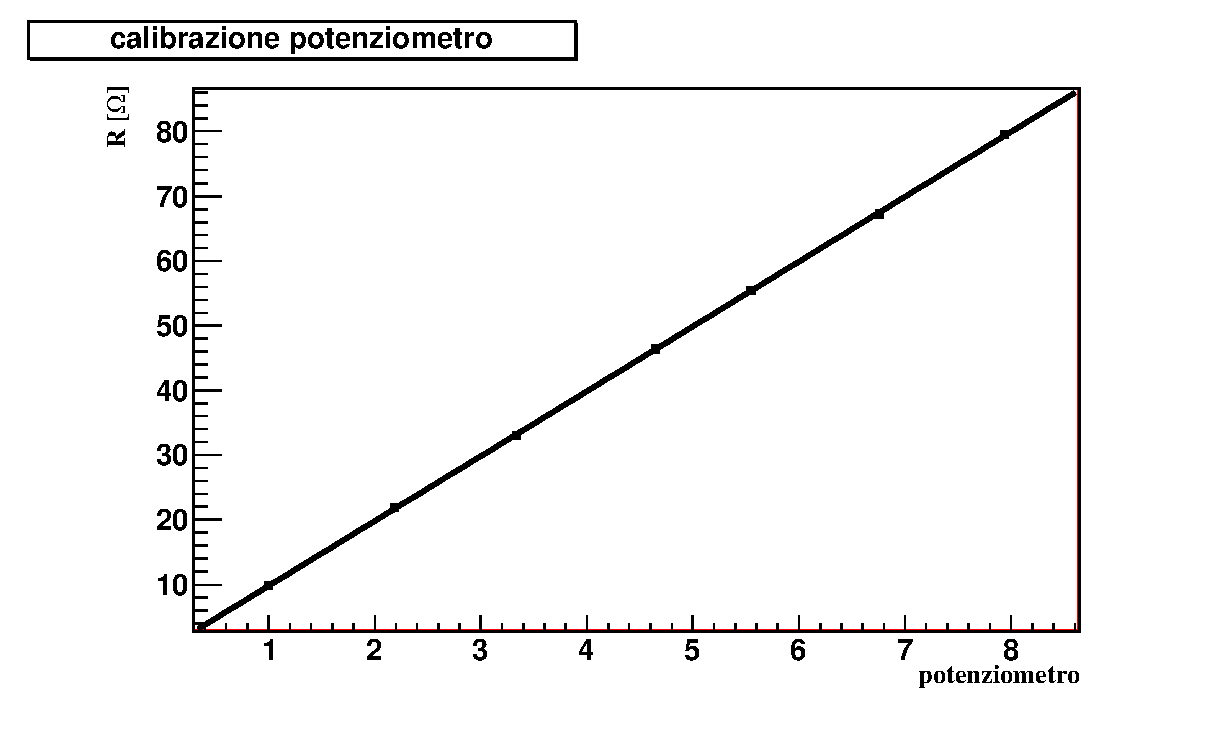
\includegraphics[width=0.48\textwidth]{img/calibrazione.potenziometro1.oscilloscopio.eps}
        \includegraphics[width=0.48\textwidth]{img/calibrazione.potenziometro2.eps}
    \end{center}
    \caption{Punti di calibrazione e rette interpolanti per i due
    potenziometri. Le barre di errore sono più piccole delle dimensioni dei
    punti.}
    \label{fig:potenziometri}
\end{figure}


\subsection{Amplificatore selettivo}
L'amplificatore selettivo aumenta l'ampiezza del segnale solo per frequenze molto vicine alla frequenza di risonanza.
\`E quindi necessario ricavare la curva di risonanza dell'apparato, mostrata
in figura \ref{fig:risonanza}. I punti --- riportati in tabella
\ref{tab:risonanza} --- sono stati interpolati con la funzione
\begin{equation*}
    A(\nu) = \dfrac{a}{\sqrt{1+b(\nu^2-\nu_{0}^2)^2}}
\end{equation*}
Il valore del parametro $\nu_0$ restituisce la frequenza del picco di
risonanza.
\begin{equation*}
    \nu_0 = \unit[564 \pm 7]{Hz}
\end{equation*}

\begin{figure}[h]
    \centering
        \includegraphics[width=0.7\textwidth]{img/risonanza.eps}
    \caption{Curva di risonanza per l'amplificatore selettivo, interpolante
    le misure di ampiezza del segnale amplificato in funzione della frequenza
    del generatore. La barre di errore sono presenti ma poco visibili.}
    \label{fig:risonanza}
\end{figure}
 
\subsection{Termometro di controllo}
Per monitorare la temperatura della camera da vuoto si è inserita al suo
interno una resistenza di controllo\footnote{Il valore restituito dal
termometro di controllo in cortocircuito 
\begin{equation*}
    R_{cc} = \unit[0.9 \pm 0.2]{\ohm}
\end{equation*}
è stato da qui in avanti sottratto in ogni misura.} $\RC$.
Sono stati portati
i capi all'esterno, collegandoli al multimetro. Accendendo la pompa a vuoto e successivamente il compressore
sono state fatte misure di temperatura al variare del tempo, sia con il termometro di
controllo sia con il termometro del campione $\RT$.
Utilizzando la tabella di conversione da resistenza a temperatura fornita
con lo strumento è stata
realizzata la curva di raffreddamento per i due termometri, riportata in
figura~\ref{fig:tempo_T} e~\ref{fig:tempo_Tc}. Infine, con il riscaldatore
ausiliario, alimentato con una potenza di \unit[25]{W}, abbiamo riportato il
campione a una temperatura di circa \unit[220]{K}.
\begin{figure}[h!]
    \centering
        \includegraphics[width=0.5\textwidth]{img/tempo_pressione.eps}
    \caption{Pressione in funzione del tempo nella camera a vuoto.}
    \label{fig:tempo_pressione}
\end{figure}

\begin{figure}[h!]
    \centering
        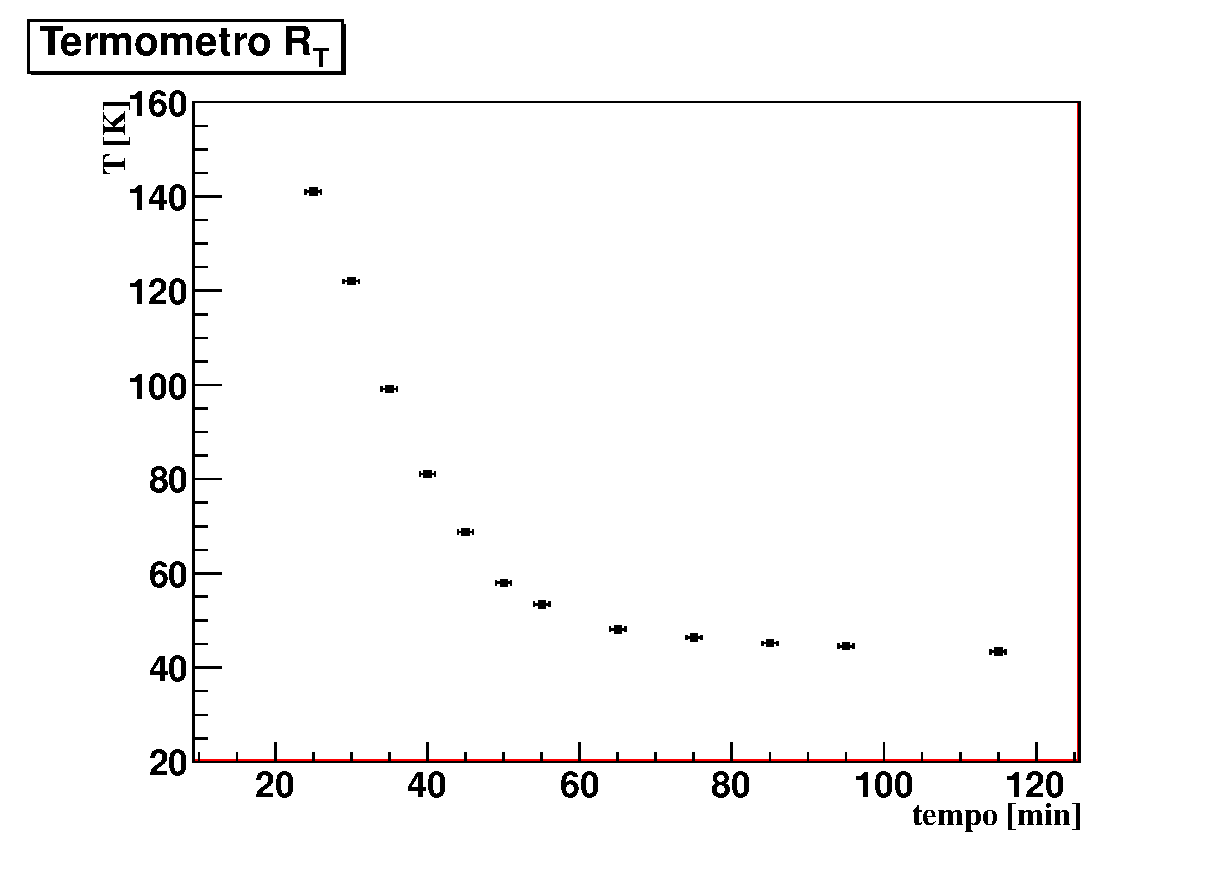
\includegraphics[width=0.5\textwidth]{img/tempo_T.eps}
    \caption{Temperatura del campione in funzione del tempo.}
    \label{fig:tempo_T}
\end{figure}

\begin{figure}[h!]
    \centering
        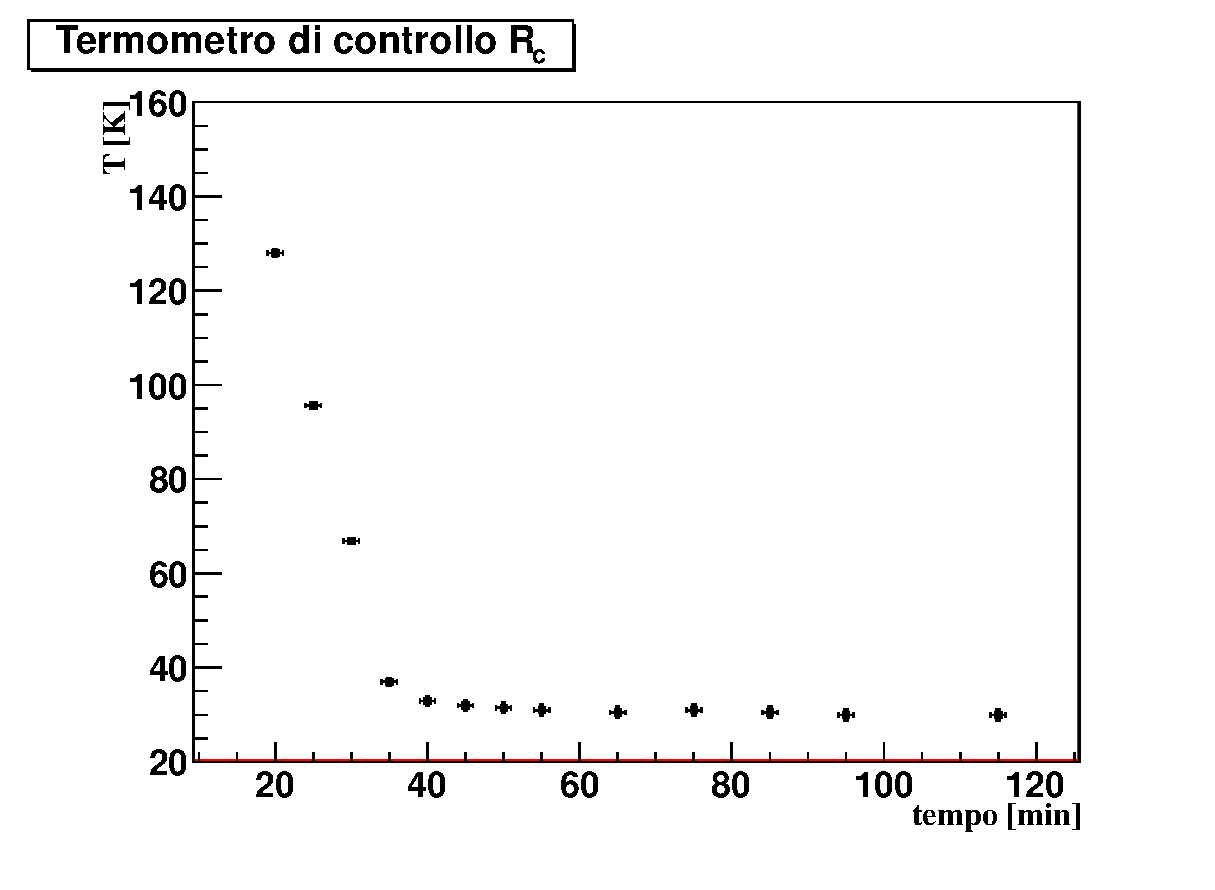
\includegraphics[width=0.5\textwidth]{img/tempo_Tc.eps}
    \caption{Temperatura del termometro di controllo in funzione del tempo.}
    \label{fig:tempo_Tc}
\end{figure}

\subsection{Inserimento del campione}
Conclusi il montaggio e la calibrazione dell'elettronica, è stato inserito
il filo di rame, ovvero la resistenza $\RD$. Si è scelta una lunghezza di $\unit[11]{m}$, in modo da avere una resistenza
a temperatura ambiente attorno ai $\unit[90]{\ohm}$. Per ottenere tale valore
si è partiti dalla relazione tra resistenza $R$ e resistività $\rho$
\begin{equation}
    \rho = R \dfrac{S}{L}
    \label{resistenza-resistività}
\end{equation}
dove $S$ è la sezione del filo ed $L$ la lunghezza. Per il filo utilizzato
si ha
\begin{center}
    \begin{tabular}{r@{ = }l}
        $\rho(\unit[293]{K})$ & \unit[$1.69 \cdot 10^{-8}$]{\ohm m} \\
           $d$    & \unit[50]{\micro m} \\
    \end{tabular}
\end{center}

Si è quindi effettuato un test dell'apparato a temperatura ambiente. Il
valore misurato col multimetro è
\begin{equation*}
    \RD = \dfrac{\rho l}{A} = \unit[84.8 \pm 0.5]{\ohm}
\end{equation*}
da correggere, sottraendo la resistenza dei fili di collegamento $R_\text{fili} =
\unit[1.40]{\ohm}$, e quella di cortocircuito:
\begin{equation*}
    \RD^\text{corretto} = \unit[83.2 \pm 0.5]{\ohm}
\end{equation*}
La misura del potenziometro ---convertita in resistenza--- restituisce
invece
\begin{equation*}
    \RND = \unit[82.8 \pm 0.2]{\ohm},
\end{equation*}
compatibile entro gli errori con il valore precedente.


\clearpage
\section{Misura della temperatura di Debye}
Sono state prese misure di resistenza in funzione della temperatura (tabella
\ref{tab:temperatura_resistenza_debye} e figura
\ref{fig:temperatura_resistenza_debye}) per ottenere una stima della
temperatura di Debye del rame attraverso la formula
semi-empirica di Bloch-Gr\"uneisen 
\begin{equation}
    \rho (T) = A \left( \dfrac{T}{\td} \right)^5 \int_0^\frac{\td}{T}
    \dfrac{x^5 e^x}{(e^x-1)^2} \diff x
    \label{bloch-gruneisen}
\end{equation}
dove \td{} è la temperatura di Debye e $A$ è una costante che dipende dal
metallo. 

\begin{figure}[h!]
    \centering
        \includegraphics[width=0.6\textwidth]{img/temperatura_resistenza_debye}
        \caption{Resistenza del filo di rame in funzione della temperatura.}
    \label{fig:temperatura_resistenza_debye}
\end{figure}


\subsection{Metodo del $\chi^2$ per l'analisi dati}
Per confrontare l'andamento teorico con i dati sperimentali è stata usata la
funzione $\chi^2$, trovando i valori di $A$ e \td{} che la minimizzano. La
funzione è definita come
\begin{equation}
    \chi^2 (A ,\td) = \sum_i \dfrac{[\rs(T_i) - \rt(T_i, A, \td)]^2}{\sigma_i^2}  
    \label{chi2}
\end{equation}
dove gli $\rs$ sono i valori misurati alle diverse temperature con errore
$\sigma$, mentre gli $\rt$ sono quelli
calcolati a partire dalla \eqref{bloch-gruneisen} alle stesse temperature, in funzione di $A$ e $\td$. 

Per passare dalla resistenza del filo alla resistività del rame si
usa la relazione \eqref{resistenza-resistività}. Se costante, il rapporto $D
\equiv S/L$ può essere inglobato in $A$, ma la presenza di variazioni
dovute alle contrazioni termiche rendono necessaria una stima dell'entità
dell'effetto.
Essendo $\rho$ prodotto di $R(T)$ e $D(T)$, è sufficiente un confronto
tra l'errore statistico relativo sulle misure e la variazione
relativa dovuta alla dilatazione termica. 
Quest'ultima dipende linearmente dalla
temperatura per un solido\footnote{In realtà a temperatura molto basse la lunghezza è quasi
indipendente dalla temperatura, ma questo rende l'effetto a maggior ragione
trascurabile. Inoltre la legge è un'approssimazione al primo ordine, in
quanto $D$ è rapporto di un'area (che scala come $1+2\alpha \Delta T$) e di
una lunghezza (che scala come $1+\alpha \Delta T$). Sviluppando in serie,
al primo ordine si ha proprio la \eqref{dilatazione_termica}.},
secondo la legge
\begin{equation}
    \dfrac{D}{D_0} = 1 + \alpha (T-T_0) \longrightarrow \dfrac{\Delta_D}{D_0} = \alpha (T-T_0)
    \label{dilatazione_termica}
\end{equation}
dove la \emph{costante di
dilatazione termica} $\alpha=\unit[17\cdot 10^{-6}]{K^{-1}}$ per il rame,
mentre $T_0 = \unit[293]{K}$.  
In tabella \ref{tab:temperatura_resistenza_debye} sono riportati l'errore percentuale
sulle resistenze e la variazione percentuale di $D$. Si vede come l'effetto
di dilatazione termica sia sempre minore dell'errore percentuale sulle
misure, e per questo in prima analisi è stato trascurato.

Il valore $\bar{A}$ che minimizza la \ref{chi2} può essere trovato
analiticamente, da
\begin{equation*}
    \dfrac{\partial \chi^2}{\partial A}(\bar{A}) = 0.
\end{equation*}
Definendo $\rtrid$ in modo che $\rt(T, A, \td) = A \rtrid(T,
\td)$, si isola la dipendenza da $A$. Riscrivendo la formula per il
$\chi^2$ usando $\rtrid$ risulta:
\begin{equation*}
    \bar{A}(\td) = \frac{S_1}{S_2}, \qquad \text{con}\quad 
    S_1= \sum_i \dfrac{\rtrid(T_i)}{\sigma_i^2}, \quad 
    S_2= \sum_i \dfrac{\rs(T_i) \rtrid(T_i)}{\sigma_i^2}
\end{equation*}

A questo punto abbiamo trovato la dipendenza $A(\td)$, che va sostituita in
\ref{chi2}. Il valore di $\td$ che minimizza $\chi^2$ non può essere trovato
analiticamente. Assegnando diversi
valori a $\td$ è possibile calcolare $\chi^2(\td)$ e disegnare la funzione per
punti. Una volta selezionato un intervallo in cui si trova il minimo si
infittiscono i punti, determinando infine l'ascissa esatta con un fit
parabolico nella zona più prossima al minimo. Più nel dettaglio, la valutazione grossolana è stata fatta con
passo \unit[1]{K} nell'intervallo $[\unit[300]{K}, \unit[400]{K}]$ --- in cui è noto trovarsi
il valore atteso di $\td$ --- mentre quella fine con
passo \unit[0.1]{K} nell'intervallo $[\unit[338]{K}, \unit[348]{K}]$.

L'errore da attribuire al valore di minimo si calcola tenendo conto che la
distribuzione del $\chi^2$ è gaussiana, e pertanto ha una deviazione
standard $\sigma = 2N$, con $N$ numero di misure. Partendo dal valore minimo
e salendo di $\sigma$ in ordinata (cfr. figura \ref{fig:chi2}) si trovano i
due punti di intersezione con la curva $\theta_{d1}$ e $\theta_{d2}$, la cui semidistanza
sarà l'errore da attribuire a $\td$:
\begin{equation*}
    \sigma_{\td} = \dfrac{\theta_{d1} - \theta_{d2}}{2}
\end{equation*}

\begin{figure}[h!]
    \centering
    \subfigure[Divisione 1 pto/K]{\includegraphics[width=0.47\textwidth]{img/chi2}}
    \subfigure[Divisione 10 pti/K ed errore]{\includegraphics[width=0.47\textwidth]{img/chi2_dettagliato}}
    \caption{Valori della funzione $\chi^2$ per diverse temperature $\td$.}
    \label{fig:chi2}
\end{figure}


\subsection{Risultati}
L'analisi precedente fornisce una stima della temperatura di Debye
\begin{equation*}
    \td = 341.7 \pm \unit[2.5]{K}
\end{equation*}
da confrontarsi con un valore di riferimento in letteratura, come\footnote{Kittel, \emph{Introduction to
    Solid State Physics} 7th ed., Wiley, pag.~126.}
\begin{equation*}                    
    \td^{\text{Kittel}} = \unit[343]{K}
\end{equation*}

Per verificare la bontà dell'approssimazione fatta sulla dilatazione
termica è stata rieseguita l'analisi, correggendo i valori misurati. Più
precisamente, dal momento che la resistività è stata sovrastimata a
temperature minori di quella dell'ambiente, sono stati diminuiti i valori di resistenza di una
percentuale pari a quella riportata in tabella \ref{tab:temperatura_resistenza_debye}.
Questa analisi porta allo stesso valore della temperatura di Debye, quindi
l'approssimazione è effettivamente buona.

Per controllare l'andamento dei dati alle diverse temperature, le misure sono
state suddivise in 3 gruppi, rispettivamente a basse, medie e alte temperature.
L'analisi condotta, analoga alla precedente, si può apprezzare in figura
\ref{fig:debye3intervalli} e restituisce i seguenti valori di minimo:
\begin{center}
    \begin{tabular}{cr@{ $\pm$ }l}
        Intervallo [K] & \multicolumn{2}{c}{$\td$}  \\
        \hline
        30--80 & 315.4 & \unit[12.2]{K}  \\
        80--170 & 340.6 & \unit[4.0]{K} \\
        170--270 & 362.6 & \unit[8.6]{K}  \\
    \end{tabular}
\end{center}

\begin{figure}[h!]
    \centering
    \subfigure[30--80 K]{\includegraphics[width=0.3\textwidth]{img/chi2__low}}
    \subfigure[80--170 K]{\includegraphics[width=0.3\textwidth]{img/chi2__med}}
    \subfigure[170--270 K]{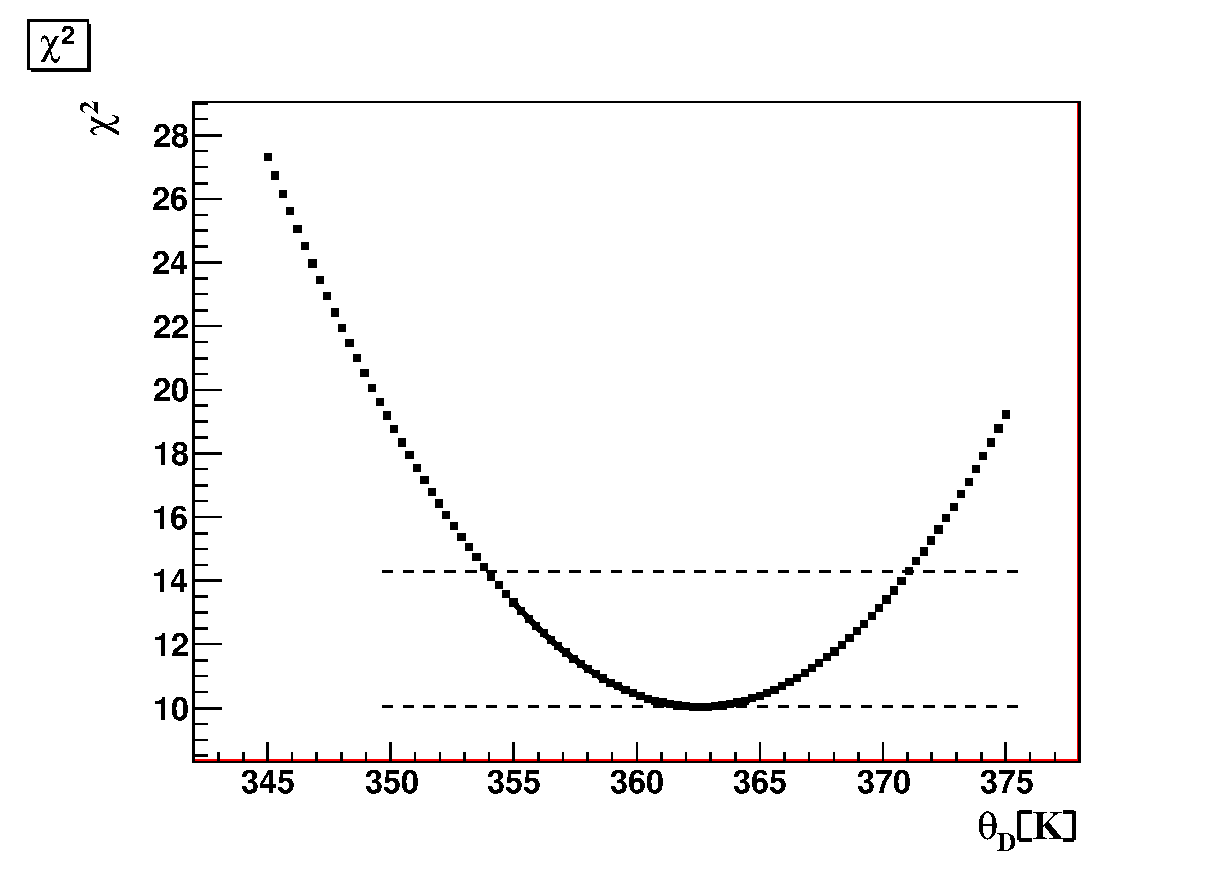
\includegraphics[width=0.3\textwidth]{img/chi2__high}}
    \caption{Metodo del $\chi^2$ per determinare $\td$ a partire dai dati
    provenienti da diversi intervalli di temperature.}
    \label{fig:debye3intervalli}
\end{figure}

\clearpage
\section{Appendice}
\subsection{Calcolo errori}
Per resistenza interna si intende quella ottenuta cortocircuitando le punte
metalliche usate per le misure. Tale valore è stato sottratto in ogni misura
diretta di resistenza.
\begin{itemize}
    \item \textsc{Multimetro GDM} \\
        Errori:
\begin{center}
    \begin{tabular}{l@{ : }r@{ + }l}
         $\unit[20]{\ohm}$   & $\unit[1]{\%}$  & $\unit[2]{dgt}$ \\
         $\unit[200]{\ohm}$ & $\unit[0.2]{\%}$  & $\unit[2]{dgt}$ \\
         $\unit[2K\ohm \rightarrow 2]{M\ohm}$ & $\unit[0.2]{\%}$  & $\unit[2]{dgt}$ \\
    \end{tabular}
\end{center}
        Resistenza interna:
        \begin{equation*}
            R_\text{int}  = \unit[0.2]{\ohm}
        \end{equation*}
    \item \textsc{Multimetro Wavetek} \\
        Errori:
\begin{center}
    \begin{tabular}{l@{ : }r@{ + }l}
        $\unit[200]{\ohm} \rightarrow \unit[2]{M\ohm}$ & $\unit[1]{\%}$  & $\unit[4]{dgt}$ \\
    \end{tabular}
\end{center}
        Resistenza interna:
        \begin{equation*}
            R_\text{int}  = \unit[0.15]{\ohm}
        \end{equation*}
    \item \textsc{Oscilloscopio} \\
        Errore sulle tensioni: \unit[2]{\%}.
\end{itemize}

\clearpage
\subsection{Tabelle}

\begin{table}[htb]
    \centering \small
    \input{tab/risonanza}
    \caption{Valori di ampiezza del segnale e frequenza del generatore con
    cui si è costruita la curva di risonanza.}
    \label{tab:risonanza}
\end{table}
\begin{table}[htb]
    \centering \small
    \input{tab/tempo-P-T}
    \caption{Misure di pressione e temperatura in funzione del tempo. La
    temperatura $T$ è quella ottenuta dal potenziometro $\RNT$, mentre $T_c$
    è quella del termometro di controllo $R_c$.}
    \label{tab:tempo-P-T}
\end{table}
\begin{table}[htb]
    \centering \small
    \begin{tabular}{r@{ $\pm$ }lr@{ $\pm$ }l|cc}
\multicolumn{2}{c}{$\unit[T]{[K]}$} &\multicolumn{2}{c}{$\unit[R]{[\ohm]}$} & $\sigma_R/ R$ [\%] &  $\Delta_D / D$ [\%] \\
 \hline
32.4 & 0.5 & 0.59 & 0.10 & 17.64 & 0.44 \\ 
 32.9 & 0.5 & 0.59 & 0.10 & 17.64 & 0.44 \\ 
 34.2 & 0.4 & 0.79 & 0.10 & 13.11 & 0.44 \\ 
 35.4 & 0.4 & 0.89 & 0.10 & 11.62 & 0.44 \\ 
 37.3 & 0.4 & 1.10 & 0.10 & 9.47 & 0.43 \\ 
 39.5 & 0.4 & 1.20 & 0.10 & 8.67 & 0.43 \\ 
 41.5 & 0.3 & 1.40 & 0.10 & 7.42 & 0.43 \\ 
 44.0 & 0.3 & 1.61 & 0.10 & 6.48 & 0.42 \\ 
 46.6 & 0.3 & 1.91 & 0.10 & 5.45 & 0.42 \\ 
 48.6 & 0.3 & 2.01 & 0.10 & 5.17 & 0.42 \\ 
 52.1 & 0.3 & 2.42 & 0.10 & 4.30 & 0.41 \\ 
 57.5 & 0.3 & 3.64 & 0.10 & 2.87 & 0.40 \\ 
 60.0 & 0.3 & 4.25 & 0.10 & 2.46 & 0.40 \\ 
 62.4 & 0.3 & 4.86 & 0.10 & 2.15 & 0.39 \\ 
 67.6 & 0.3 & 6.29 & 0.10 & 1.67 & 0.38 \\ 
 71.4 & 0.3 & 7.30 & 0.11 & 1.44 & 0.38 \\ 
 75.6 & 0.3 & 8.42 & 0.11 & 1.26 & 0.37 \\ 
 79.1 & 0.3 & 9.13 & 0.11 & 1.16 & 0.36 \\ 
 85.3 & 0.3 & 11.57 & 0.11 & 0.93 & 0.35 \\ 
 88.1 & 0.3 & 12.49 & 0.11 & 0.86 & 0.35 \\ 
 90.8 & 0.3 & 13.41 & 0.11 & 0.81 & 0.34 \\ 
 94.2 & 0.3 & 14.63 & 0.11 & 0.74 & 0.34 \\ 
 99.6 & 0.3 & 16.46 & 0.11 & 0.67 & 0.33 \\ 
 109.0 & 0.3 & 19.51 & 0.11 & 0.58 & 0.31 \\ 
 115.0 & 0.3 & 21.54 & 0.11 & 0.53 & 0.30 \\ 
 119.0 & 0.3 & 22.86 & 0.12 & 0.50 & 0.30 \\ 
 126.0 & 0.3 & 25.41 & 0.12 & 0.46 & 0.28 \\ 
 132.0 & 0.3 & 27.44 & 0.12 & 0.44 & 0.27 \\ 
 136.0 & 0.3 & 29.07 & 0.12 & 0.42 & 0.27 \\ 
 146.0 & 0.3 & 32.02 & 0.12 & 0.39 & 0.25 \\ 
 153.0 & 0.4 & 34.66 & 0.13 & 0.37 & 0.24 \\ 
 160.0 & 0.4 & 37.00 & 0.13 & 0.35 & 0.23 \\ 
 169.0 & 0.4 & 40.26 & 0.14 & 0.34 & 0.21 \\ 
 173.0 & 0.4 & 41.07 & 0.14 & 0.33 & 0.20 \\ 
 177.0 & 0.4 & 42.50 & 0.14 & 0.33 & 0.20 \\ 
 181.0 & 0.4 & 43.72 & 0.14 & 0.32 & 0.19 \\ 
 194.0 & 0.4 & 47.99 & 0.15 & 0.31 & 0.17 \\ 
 204.0 & 0.5 & 51.45 & 0.15 & 0.30 & 0.15 \\ 
 216.0 & 0.5 & 55.31 & 0.16 & 0.29 & 0.13 \\ 
 223.0 & 0.5 & 57.65 & 0.16 & 0.28 & 0.12 \\ 
 234.0 & 0.5 & 61.41 & 0.17 & 0.27 & 0.10 \\ 
 245.0 & 0.5 & 65.08 & 0.17 & 0.27 & 0.08 \\ 
 265.0 & 0.6 & 71.99 & 0.19 & 0.26 & 0.05 \\ 
 \end{tabular}
    \caption{Resistenza del filo di rame in funzione della temperatura della
    camera. Le misure, fatte con i potenziometri, sono state convertite in
    resistenze $\RD$ ed $\RT$, e quest'ultima poi in temperatura.}
    \label{tab:temperatura_resistenza_debye}
\end{table}

\clearpage
\subsection{Grafici}
\begin{figure}[tp]
    \centering
        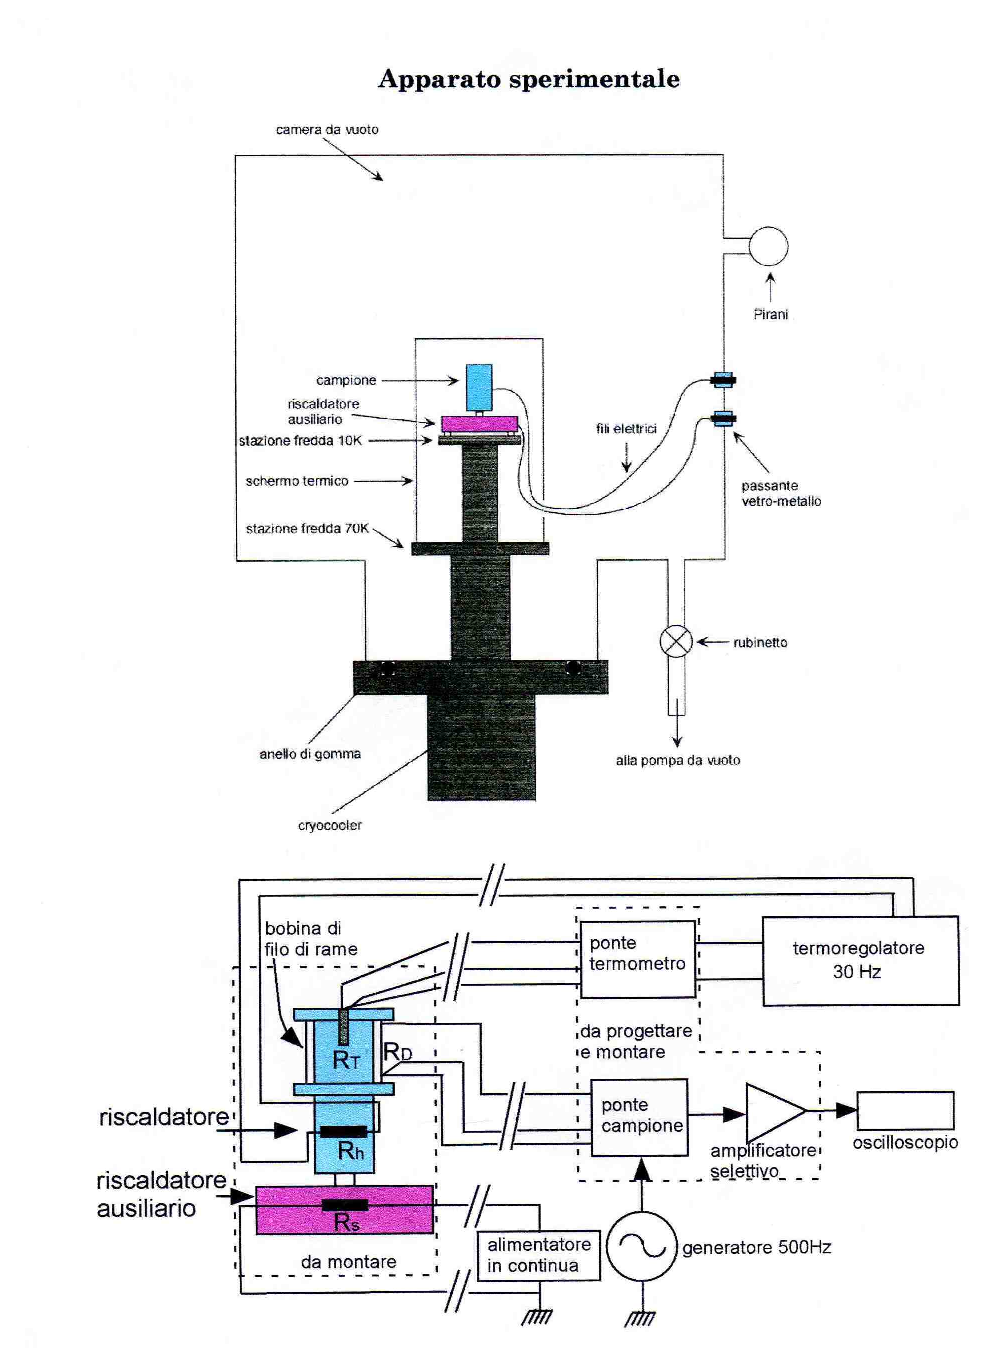
\includegraphics[width=0.9\textwidth]{img/apparato.sperimentale.eps}
    \caption{Descrizione schematica dell'apparato sperimentale.}
    \label{fig:apparato}
\end{figure}

\begin{figure}[tp]
    \centering
        \includegraphics[width=0.9\textwidth]{img/ponte.rt.eps}
    \caption{Ponte di Wheatstone per la misura della temperatura.}
    \label{fig:rt}
\end{figure}
\begin{figure}[tp]
    \centering
        \includegraphics[width=0.9\textwidth]{img/ponte.rd.eps}
    \caption{Ponte di Wheatstone per la misura della resistenza $\RD$.}
    \label{fig:rd}
\end{figure}
\begin{figure}[tp]
    \centering
        \includegraphics[width=0.9\textwidth]{img/ampli.selettivo.eps}
    \caption{Rappresentazione schematica dell'amplificatore selettivo.}
    \label{fig:ampli.selettivo}
\end{figure}

\end{document}
